One way of implementing a parallel scan is with the algorithm developed by Hillis and Steele \cite{Hillis:1986:DPA:7902.7903}. This implementation is also called the naive parallel scan, because of its work inefficiency. A visual representation of the algorithm is show in \cref{fig:scan_hillis_steele}. 

\begin{figure}[ht]
	\centering
	\fbox{
		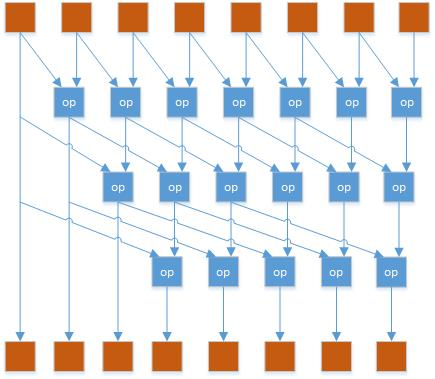
\includegraphics[width=0.4\textwidth]{figs/algorithm/scan_hillis_steele.jpg}}
	\caption{TBD}
	\label{fig:scan_hillis_steele}
\end{figure}

The algorithm iterates through $log n$ steps, where n is the number of array elements to sum. At each step each element is combined through the binary associative operator with its right $ 2^k $ neighbour, where k is the step depth starting at zero. The Hillis/Steele is natively a inclusive scan but can be implemented as an exclusive scan e.g. by shifting. The step complexity of the Hillis/Stelle scan is $O(log n)$, thereby being step efficient. The work complexity on the other hand is $O(n log n)$, making it work inefficient. The algorithm assumes that there is as many processors in the system as there is data elements to be combined, this is not always the case. For small array sizes the Hillis/Steele scan is on the other hand efficient, as it will keep the processors busy, and create the result in few steps. 

[TODO: overvej kode]  